\documentclass[11pt]{article}
\usepackage[top=1in, bottom=1in, left=1in, right=1in]{geometry}
\usepackage{graphicx}
\usepackage{amsfonts, amsmath, amssymb}
\graphicspath{{./images/}}
\renewcommand{\baselinestretch}{1.5}
\begin{document}
\thispagestyle{empty}
\begin{center}
\Huge{}math seminars\\
\begin{figure}
\center{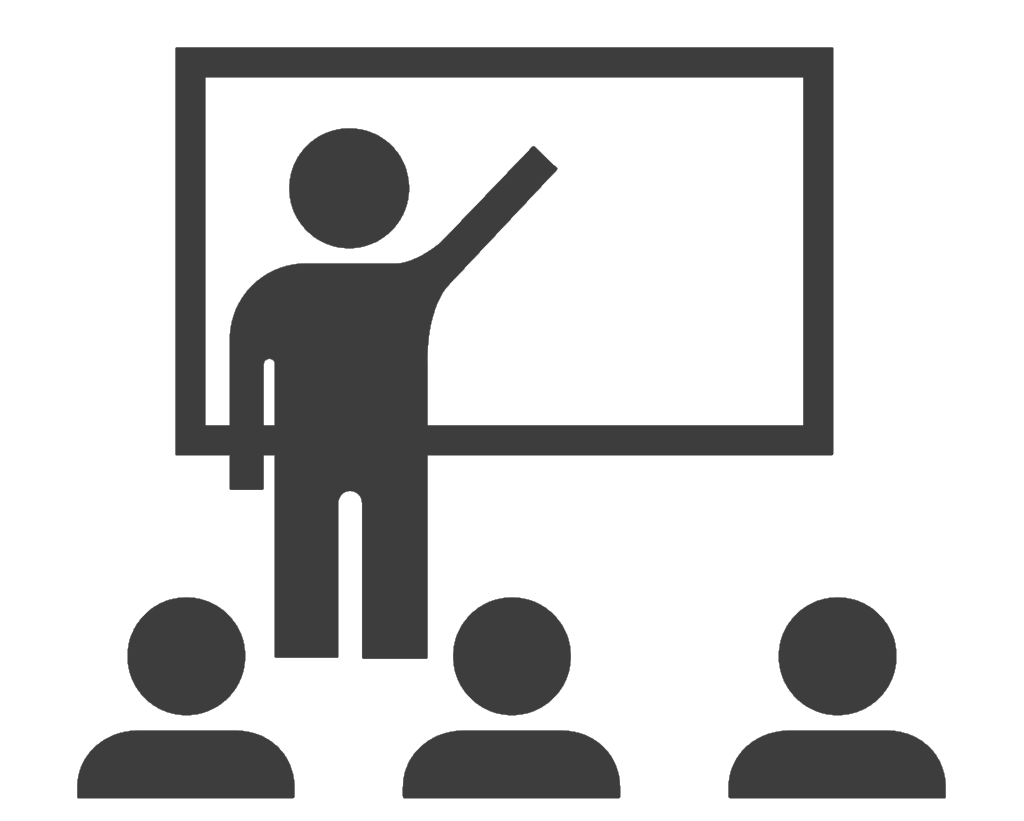
\includegraphics[scale=0.33]{lol}}
\end{figure}
\Large{} A small group for doing cool math with lectures and discussions\\
\end{center}
We are not affiliated with MA$\Theta$. Join us in group sessions where students (yes, \textit{you}) can volunteer to talk about math we don't get to learn at school. This group is semi-informal, fun, and is entirely interest-based.\vspace{5pt}\\
The first meeting will be an informational meeting after school in Mr. Doherty's room (portable 807), on \textbf{Wednesday, September 4th} until at most 4:30 PM. We will clarify questions and form the meetings calendar for the next few months. If you are thinking of lecturing, please come with a few ideas and available dates beforehand, so we can form the calendar efficiently. This will be the only required meeting.\vspace{5pt}\\
We want to include as many people as possible in the group, so there are no formal requirements regarding prerequisite mathematical knowledge, so lecturers have to prepare appropriate content. Acceptable topics include stuff from linear algebra, multivariable/vector calculus, real/complex analysis, number theory, differential equations (ODE/PDE), combinatorics, geometry, and statistics, to name a few. Anything accessible from an undergraduate mathematics education is fine. 
\begin{flushright}
Questions? Ask Mr. Doherty or Sai Sivakumar
\end{flushright}
\end{document}